% Save LaTeX kernel version of \@xfloat
\makeatletter
\let\my@xfloat\@xfloat
\makeatother
\documentclass[%
        %draft,
        %submission,
        compressed,
        final,
        %
        %technote, 
        %internal,
        %submitted,
        %inpress,
        %reprint,
        %
        %titlepage,
        notitlepage,
        %anonymous,
        narroweqnarray,
        inline,
        twoside,
        ]{ieee}

% Reset to LaTeX kernel version of \@xfloat 
\makeatletter
\def\@xfloat#1[#2]{
\my@xfloat#1[#2]% 
\def\baselinestretch{1}%
\@normalsize \normalsize
}
\makeatother
%	
% some standard modes are:
%
% \documentclass[draft,narroweqnarray,inline]{ieee}
% \documentclass[submission,anonymous,narroweqnarray,inline]{ieee}
% \documentclass[final,narroweqnarray,inline]{ieee}

% Use the `endfloat' package to move figures and tables to the end
% of the paper. Useful for `submission' mode.
%\usepackage {endfloat}
 
% Use the `times' package to use Helvetica and Times-Roman fonts
% instead of the standard Computer Modern fonts. Useful for the 
% IEEE Computer Society transactions.
% (Note: If you have the commercial package `mathtime,' it is much
% better, but the `times' package works too).
%\usepackage {times}

% In order to use the figure-defining commands in ieeefig.sty...

\usepackage{tikz}
\usepackage{graphicx}
\usepackage{amsmath}
\usepackage{amsfonts}
\usepackage{float}
%\usepackage{url}
\usepackage{biblatex}
\bibliography{mybib.bib}

\usepackage[utf8]{inputenc}

%\usepackage{ieeefig}

\title{A study on the classification of handwritten digits}
\author{Laurent Verweijen, \and Tamis van der Laan}
\date{January 14, 2013}

\begin{document}
\maketitle

\begin{abstract}
This paper describes our research for using pattern recognition techniques to
classify individual digits in bank account numbers and the monetary amount. This
paper will describe the steps we have taken to do such a task which consists of
preprocessing the data, training the classifier and testing the performance.
Matlab was used to perform these steps. Two cases are taken into account. In the
first case the pattern recognition system is trained once and then applied.
That means that our training set is large. In the second case, the training set
is trained for each batch to be processed, which means that our training set is
much smaller. We describe how we found the optimal classifiers, how these
classifiers work and how we optimized these classifiers to make them perform
even better. After doing a lot of tests, we noticed that the best performance
for the small dataset was reached by using a nearest mean scaled classifier and
for the big dataset the voted perceptron classifier performed best. 
\end{abstract}

\section{Introduction}
In our approach Matlab was used to research these problems using the PR toolbox
for fast prototyping. 
This toolbox contains common classifiers used for pattern recognition which
include among others the support vector machine and the k-nearest-neighbour
classifier. 
The PR toolbox for Matlab was developed by the Delft Pattern Recognition Group
(in 2004 renamed to Quantitative Imaging) at the Faculty of Applied Physics
(later Applied Sciences) of Delft University of Technology \cite{Ferdi}.
We will first
discuss how we solved the first case, then the second case and finally we will
give some conclusions and recommendations about how this could be applied in a
banking system. Prior experience with person recognition \cite{Tamis} led us to
the use of Histogram of Oriented Gradients feature
extraction in combination with a support vector machine classifier. Eventually
the support vector machine would be dropped in favor of a similar less
computationally expensive classifier named the voted perceptron classifier. Many
other classifiers were also tested. For the second case where the data set was
small we found that the nearest nearest mean scaled classifier performed best.

\section{Methods}
\subsection{Pre-processing}
Either before training or classification a preprocessing step is used in order
to filter out noise and transform the image in such a way that structure is
maintained and the data is prepared for feature selection, extraction and
classification. Initially the data that was provided consisted of a set of
images from different sizes that each contains a handwritten digit.

\begin{figure}[h!]
    \centering
    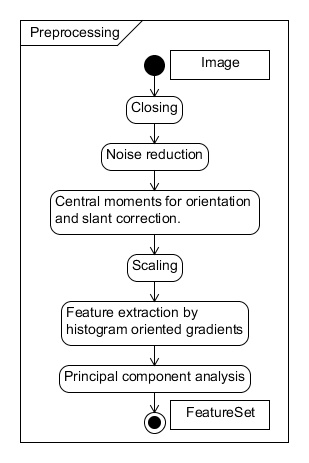
\includegraphics[width=\columnwidth]{preprocessing2.png}
    \caption{Preprocessing pipeline}
    \label{fig:preprocessing}
\end{figure}

Figure \ref{fig:preprocessing} shows the pipeline that was used for preprocessing. First noise is reduced by removing very small objects. Then the data is closed in case the image contains gaps. Then the data is skewed so the longest side of the data (side with the most variance) is parallel to the y axis (slant correction). Then the features of our data are extracted and finally principal component analysis is used to reduce the size of the feature set as some features are barely to not used.\\\\
In table \ref{tab:noise_reduction} some examples that show noise reduction and slant correction
are shown based on the scheme above.
\begin{table}
    \begin{tabular}{|c|c|}
        \hline
        Before & After \\
        \hline
    
\includegraphics[width=.4\columnwidth]{images/dirty5.png}
    &
\includegraphics[width=.4\columnwidth]{images/clean5.png}\\
    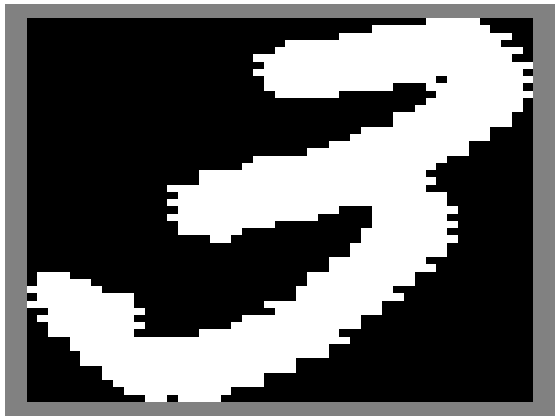
\includegraphics[width=.4\columnwidth]{images/dirty3.png}
    &
\includegraphics[width=.4\columnwidth]{images/clean3.png}\\
        %\begin{figure}
            %
\includegraphics[width=.3cm]{images/clean5.png}
        %\end{figure}
        % hier plaatjes includen
        \hline
    \end{tabular}
    \label{tab:noise_reduction}
    \caption{Noise reduction and slant correction applied to our images}
\end{table}

\subsubsection{Dilation and Erosion}

Noise is reduced by first eroding and then dilating the given binary input image
using a 2-dimensional diamond shaped kernel. We then wish to close holes or
attach objects near each other
as parts of numbers may be missing. We do this using a closing operation which
consists of a dilation followed by an erosion again using a 2-dimensional diamond shaped kernel.

\subsubsection{Central Moments for orientation and slant correction}
Next we transform the binary input image such that it is centered and oriented in such a way that the longest side of the number is parallel to the y axis. The transformation used is skewing and removes the slanting from the text. This operation will also decrease the variance of the pixels as some pixels such as those in the corners will be activated less often and therefore contribute less to the number recognition system. This decrease in pixel variance propagates through to the Histogram Oriented Features. This in turn allows Principle Component Analysis to decrease the feature set significantly as we threshold out the low variance principal components. This allows for far faster training and classification performance.

We first need to center the image. To do this we find the image centroid, which is simple the mean of the x axis and the y axis:

\begin{align}
    \bar{x}&=(x_1+x_2+...+x_n)/n_x \\
    \bar{y}&=(y_1+y_2+...+y_n)/n_y
\end{align}

In order to find the orientation of binary numbers we used central moments. Central moments are calculated in the following way and make use of the centroid:

\begin{equation}
    \mu_{pq} = \sum_x \sum_y (x - \overline{x})^p(y - \overline{y})^q f(x, y)
\end{equation}

 
Next we you use this definition to compute $\mu_{20}, \mu_{21}, \mu_{11}$ which represents the x and y variance and covariance respectively. We then use these central moments to compute the orientation as followed:

\begin{equation}
    \Theta = \frac{1}{2} \arctan \left(
        \frac{2 \cdot \mu_{11}}{\mu_{20} - \mu_{02}}
    \right)
\end{equation}

We then skew the image parallel to the y axis and find the bounding box and square it where the sides are equal to the longest previous side such that geometric information is preserved. We leave a one pixel border around the bounding box because the Histogram of Oriented Gradient algorithm (as its name already suggests) makes use of the gradient (first order derivative in both the x and y direction) and thus its three part filter needs the extra one pixel space. The slant correction skew matrix is given by:

\begin{equation}
    S = \begin{pmatrix}
        1 & 0 \\
        \sin(0.5 \pi - \theta) & \cos(0.5 \pi - \theta)
    \end{pmatrix}
\end{equation}

\subsubsection{Scaling}
Finally the images are scaled to 32 by 32 pixels, ready for feature selection, extraction and classification.
\subsection{Feature extraction and selection}
We used two methods for feature extraction and selection. The first method used
is called Histogram Oriented Gradients and is a form of feature extraction and
reduction that describes the orientation of the gradient in terms of frequency. The second method used is called principal component analysis and is used to remove those histogram of oriented gradient features with the least variance, and is thus a form of feature selection or dimensionality reduction. But before arriving at these features we first tested and experimented with combinations of other features that are commonly used when dealing with handwriting detection. We list a couple of them below:\\

    \begin{enumerate}
        \item Using raw pixels as a control
        \item Image profiles
        \item Image moments such as hu moments
        \item Canny edge detector\\
    \end{enumerate}
We however found that none could compete with the histogram of oriented gradients in combination with the classifiers tested.
    \subsubsection{Raw pixels}
The simplest features that can be taken from an image are the raw pixels. This
is also the fastest feature extraction, because the only operation that needs
to be performed is the scaling of all images to the same size. We tried this for
different image sizes. Most digits got recognized well by using this method. The
error rate on a big dataset was about 10\%. In particular the digits three and five were often mixed up. We used the raw data as a control to compare features based on classification errors. 

\subsubsection{Histogram oriented features (HOG)}
Histogram of Oriented Gradients is a feature extraction and selection technique.
\cite{hog} It makes use of the image gradient, were both the orientation of the gradient and magnitude are used. Due to the binary nature of our input we will not be using the magnitude of the gradient. The first step of the Histogram Oriented Gradients algorithm is to compute the gradient of the image. This is done by taking the first derivative of the image in both the x and y direction. The method used for this is convolution with the following filters:

\begin{equation}
    [-1, 0, 1] \text{ and } [-1, 0, 1]^T
\end{equation}

We now obtain two images containing the x derivative and y derivative respectively. The direction angle of the gradient for each pixel can now be computed using the following formula: 

\begin{equation}
    \theta = \arctan\left(\frac{\partial f}{\partial y}, 
        \frac{\partial f}{\partial x}\right)
\end{equation}

The next step is to create cells which will contain histograms. In the original
paper the gradient magnitude of each pixel within the range of a given bin is
summed to get the final bin value. The original paper is aimed at pedestrian
detection however using grey scale images. Because we are using binary images we
simply increase the bin width with one if the gradient direction of a pixels lays within the range of the given bin.\\\\
This method will result in several bins per cell, the original author used 9
bins per cell and 16 cells. We found through experiment that 9 bins were most effective for
our problem as well, but 16 cells were used as opposed to 9 used by the original author.
We derived at these constants experimentally by looking at the average and
minimum error of all the tested classifiers for each possible combination were
25 cells and 10 bins were chosen as maximums. \\\\

Next, the author locally normalizes the cells in order to compensate for illumination and contrast. However we do not implement this step as we are using binary images and thus both the contrast and illumination are already normalized perfectly across our image.\\\\
The last step is to put all the bins of each cells into a column vector which has became our feature vector for classification.

\subsection{Principal component analysis}
The hog descriptor does a good job at both reducing the amount of features needed as well as extracting features that are easier to classify by the bulk of classifiers. However there will still remain features (bins) that are either always empty or are barely used. For this reason we apply Principal Component analysis, which will extract the principal components and allows us to remove those with too little variance (empty to barely filled bins).\\\\
Principal component analysis (pca) is a data reduction technique that generates a set of
principal components such that as much variance as possible between the features is maintained.  In the features which we extracted from the data, some features don't differ as much as other features. This is due to the way the numbers are usually written and the orientation correction we used in a previous step. We therefore use pca to make our feature set smaller, so that our classifier becomes faster.\\\\
The mathematical theory behind pca is as follows:
Let $X$ be a feature matrix with the rows representing different samples and the
columns representing different features.  We first subtract the mean of each
feature from the columns so that the mean of each column, becomes 0. We call
this new matrix $X_{adjusted}$. Then we do an eigenvalue decomposition of the
covariance of this matrix. $PDP^{-1}=cov(X_{adjusted})$. By sorting the
eigenvectors by corresponding eigenvalues, we can find the $L$ vectors that
contribute most to our data.  The highest eigenvalues correspond to the
eigenvectors that capture most covariance. The multiplication of our data with
these eigenvectors $X_{reduced}=P_L X_{adjusted}$ will then become our reduced feature set.\cite{Pearson}\\\\
Using principle component analysis we managed to reduce the 144 dimensions obtained from the histogram of oriented gradients feature extraction method to a mere 57 features which translates into a 60\% feature reduction! For the large data set we managed to reduce the 144 dimensional feature space to 82 which still signifies a major reduction of 43\% of the feature space! \\\\
Not only did the principal component analysis method increase performance, it also increased the classification accuracy! This is due to the reduction of useless dimensions and the elimination of problems related to the curse of dimensionality. This was especially so with the nearest scaled mean classifier as it is a density based classifier and thus is especially prone to the curse of dimensionality. On the small data set the classification error of the NSMC decreased with an impressive 80\%! The error on the large data set using the voted perceptron classifier also decreased with a percentage of 0.8\% which is also a very significant decrease given the large amount of data available.
\section{Classification Data Set}
Although we initially opted to use the support vector machine, we tested many
classifiers in order to find the classifier that would give us the best
classification result. It turned out that several classifiers were simply too
computationally expensive to test. We used the nist\_eval function provided
by the client to test all the classifiers. The support vector machine classifier
was one of these classifiers together with all neural network based classifiers
that were too computationally expensive to subject to rigorous testing and were
therefore not considered. We excluded these classifiers as we wish to provide a
certain degree of classification certainty to our client. We soon found a
similar classifier too the support vector machine called the Voted Perceptron classifier and found this to be
the most likely candidate for use in classification. This notion was confirmed in the testing phase as it
yielded the lowest error on the large data set of all classifiers considered.
For the small data set however the voted perceptron classifier performed decent
but not excellent. We found that the nearest mean scaled classifier performed
best on the small data set. For this reason we chose the VPC for case one and
the NMSC for case two. The performance of both classifiers were found to be more
than fast enough.

\subsection{Classifier Testing Phase}
We used the testing function provided by the client to test all the classifiers.
We used the default setting of a 100 samples to test on. With exclusion of the
support vector machine classifier and any neural network based classifiers. The
following two tables show the errors for the small and large data set
respectively:\\
\begin{table}
    \begin{tabular} {p{5cm}lp{1.5cm}} %{lll}
        \hline
    Classifier & Error & Execution Time 1.0e-05 * \\
        \hline
K-nearest neighbour Classifier                                              & 0.1220 & 0.4634 \\
Linear kernel Classifier                                                    & 01470  & 0.4966 \\
Decision tree Classifier                                                    & 0.8050 & 0.4635 \\
Fisher's Least Square Linear Classifier                                     & 0.1580 & 0.4635 \\
Linear Bayes Normal Classifier                                              & 0.1470 & 0.4635 \\
Linear classifier built on the KL expansion of the common covariance matrix & 0.1470 & 0.6290 \\
Logistic Linear Classifier                                                  & 0.1550 & 0.4966 \\
Naive Bayes classifier                                                      & 0.5290 & 0.5959 \\
Nearest Mean Classifier                                                     & 0.1340 & 0.4304 \\
Nearest Mean Scaled Classifier                                              & 0.1000 & 0.5959 \\
Linear perceptron classifier                                                & 0.3910 & 0.4966 \\
Polynomial Classification                                                   & 0.1580 & 0.4966 \\
Quadratic Bayes Normal Classifier                                           & 0.9000 & 0.4966 \\
Voted perceptron classifier                                                 & 0.1900 & 0.4966 \\
Uncorrelated normal based quadratic Bayes classifier                        & 0.2090 & 0.5297 \\
Random subspace combining classifier                                        & 0.9480 & 0.4966 \\
Linear classifier using PC expansion on the joint data                      & 0.1470 & 0.5628 \\
Parzen Classifier                                                           & 0.1130 & 0.4635 \\
        \hline
    \end{tabular}
    \caption{
        This table shows the error and execution time on the nist\_eval function
        which uses 100 samples per class to test the classifier. The training
        data consisted of the small data set of 10 samples per class. }
\end{table}

\begin{figure}[] 
    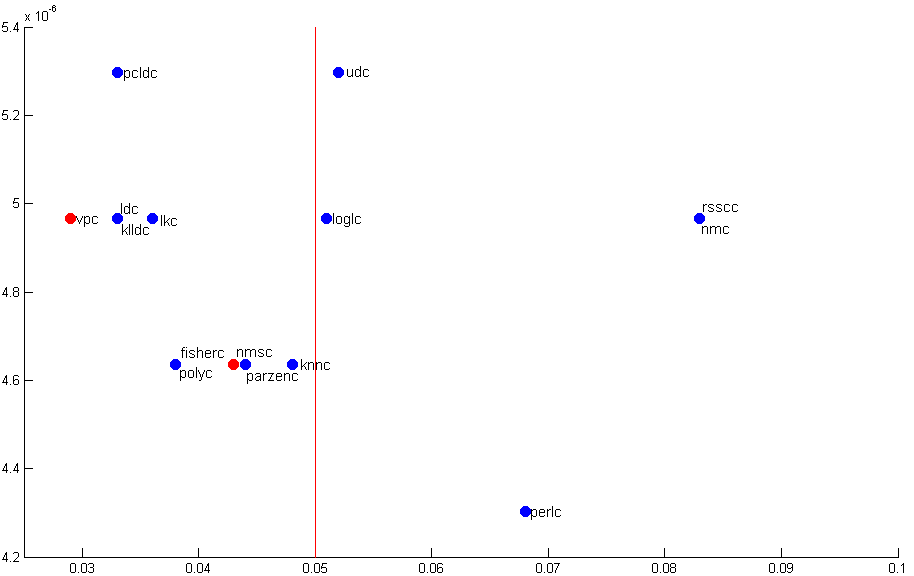
\includegraphics[scale=0.385]{images/large_data_set_tested.png}

    \caption{ This table shows the error and execution time on the nist\_eval
    function which uses 100 samples per class to test the classifier. The
training data consisted of the small data set of 10 samples per class.The
        red line shows the 25\% maximum error set by the client. }
    \label{fig:test-large}
\end{figure}

\begin{table}
    \begin{tabular} {p{5cm}lp{1.5cm}} %{lll}
        \hline
    Classifier & Error & Execution Time 1.0e-05 * \\
        \hline
K-Nearest Neighbor Classifier                                               & 0.0480 & 0.4635 \\
Linear kernel classifier                                                    & 0.0360 & 0.4966 \\
Decision Tree Classifier                                                    & 0.8030 & 0.4635 \\
Fisher's Least Square Linear Classifier                                     & 0.0380 & 0.4635 \\
Linear Bayes Normal Classifier                                              & 0.0330 & 0.4966 \\
Linear classifier built on the KL expansion of the common covariance matrix & 0.0330 & 0.4966 \\
Logistic Linear Classifier                                                  & 0.0510 & 0.4966 \\
Naive Bayes classifier                                                      & 0.1130 & 0.4304 \\
Nearest Mean Classifier                                                     & 0.0830 & 0.4966 \\
Nearest Mean Scaled Classifier                                              & 0.0430 & 0.4635 \\
Linear perceptron classifier                                                & 0.0680 & 0.4304 \\
Polynomial Classification                                                   & 0.0380 & 0.4635 \\
Quadratic Bayes Normal Classifier                                           & 0.1220 & 0.4966 \\
Voted perceptron classifier                                                 & 0.0290 & 0.4966 \\
Uncorrelated normal based quadratic Bayes classifier                        & 0.0520 & 0.5297 \\
Random subspace combining classifier                                        & 0.0830 & 0.4966 \\
Linear classifier using PC expansion on the joint data.                     & 0.0330 & 0.5297 \\
Parzen Classifier                                                           & 0.0440 & 0.4635 \\
        \hline
    \end{tabular}
    \caption{ 
        This table shows the error and execution time on the nist\_eval function
        which uses 100 samples per class to test the classifier. The training
        data consisted of the large data set of 100 samples per class. }
        
\end{table}
    
\begin{figure}[]
    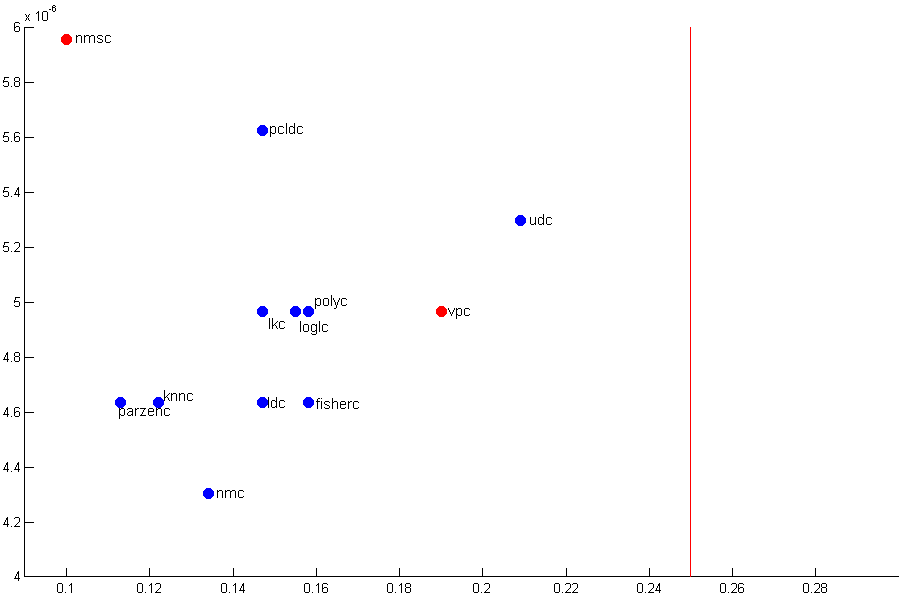
\includegraphics[scale=0.385]{images/small_data_set_tested.png}

    \caption{
        This table shows the error and execution time on the nist\_eval
    function which uses 100 samples per class to test the classifier. The
training data consisted of the large data set of 100 samples per class.The
        red line shows the 5\% maximum error set by the client.  }
    \label{fig:test-small}
\end{figure}

We see that many classifiers meet our criteria. We chose to use the two best
classifiers namely the Voted perceptron classifier for the large data set and
the Nearest Mean Scaled classifier for the small data set.

\subsection{Voted Perceptron Classifier}
As discussed above in the introduction the plan was to treat the number
recognition system in the same way as the person recognition system implemented
and described by Manabu Sassano \cite{Manabu}.
This implementation used a state vector machine for classification. But because
this classifier was too heavy for the problem at hand we opted for a simpler but
similar classifier, namely the voted perceptron classifier. This study by Manabu
Sassano, IJCNLP compared the SVM classifier to the voted perceptron classifier
and found them almost equal in terms of accuracy. The advantage however of the
Voted Perceptron Classifier is that it is significantly faster in terms of learning
and prediction time.\\\\
The Voted Perceptron Classifier is very easy to understand, let $x$ denote the
feature vector were $||x||$ denotes the amount of features and $y \in \{-1,1\}$
the corresponding label. The training algorithm simply starts by applying the
prediction step which is the simple function $\hat{y} =
sign(\overline{v}\cdot\overline{x})$ were $\overline{v}$ is
initialized at the beginning as $\overline{v}=\bar{0}$. If the prediction of $y$ is correct i.e.
$\hat{y}=y$
then no further steps are taken. If however the prediction is not correct then
the training step occurs. This training step takes the form of the following
simple equation $\bar{v}=\bar{v}+y\bar{x}$ . It has been shown that if the data is linearly separable that
the algorithm will make a finite number of mistakes but will converge after a
certain amount of cycles to the right answer. If however the data is not
linearly separable the algorithm will not converge. Therefore the amount of
cycles allowed is bounded. Due to the high performance of the algorithm we
choose the maximum amount of cycles to be 1000 which may be far more than
needed.

% TODO mooiere formules
\subsection{Nearest Mean Scaled Classifier}
The nearest mean scaled classifier is an extension of the nearest mean
classifier, so I will describe that one first.\\\\
The nearest mean classifier is a classifier that assigns a sample to the class
to which its euclidean distance is smallest. So from the training data the mean
is taking for each class and assigned to $M_C$ and then it minimizes:
\begin{equation}
    (X - M_c)^2 \text{ for $c \in C$}
\end{equation}
In which X is the feature vector from the sample that needs to be classified.
And C are the classes. $M = {M_1, …, M_k}$ are the mean vectors of all the classes
it could get assigned to.
So $M_c = \sum{x \in X \text{ for all $X \in C$}}$\\\\
The nearest mean scaling classifier is similar to a nearest mean classifier,
except that nmsc makes the assumption that the data is according to a normal
distribution, to which the data is scaled first.

\subsection{Kernel Mapping The data for classification}
The Voted Perceptron Classifier is in essence a linear classifier that can be made non linear by adding extra dimension based on the data itself. The way the data is mapped to extra dimensions is called kernel mapping, where the kernel dictates the structure of the added higher dimension. We experimented with sever proximity based kernels to construct a non linear VPC but they all yielded worse results. This suggests the data to be linear and no kernel mapping is required.

\section{Future work} 
One thing that could be researched for performance accuracy would be combining
classifiers.  For example we may be able to increase performance by
bootstrapping from the training set and training multiple voted perceptron
classifiers. We could then use the majority vote of these classifiers for
classification of given unknown samples. In this way accuracy may be increased.
We could also construct a general classifier that can classify large and small
data sets equally well by combining the VPC and the NMSC. We could again use
bootstrapping and a majority vote but this time weigh the vote by the outcome of
a function of the sample size. This function could be linear or nonlinear. A
sigmoid function might be considered. Another possibility would be to combine
the top 5 classifiers of both the small and large datasets respectively. 

\section{Conclusion and recommendations}
We have shown that by using central moments and skewing we can provide decent
text slanting correction. We also show that we can filter out noise using
erosion and dilation filters. We have also obtained desirable low level error
rates within the boundaries set by the client.\\\\
From our tests it seems like the more data is used for training the better the
results. When 1000 instead of 10 samples per class are used, the error becomes
10 times as small. However this does not mean that we will ever achieve a zero percent error rate. This is because there is a degree of subjectivity in the data, what one person may label a eight may be labeled by others as a six. We thus we see practically identical symbols in more than one class. We can only approximate with a large enough data set what class label the average person would give to a number symbol. \\\\
In this sense the system will never reach a zero percent error. Adding extra features also won't solve this problem as ambiguity can still occur. With this insight we recommend using ambiguity rejection were credit cards with ambiguous unclear numbers can be traced back to their owners by employees. \\\\
Apart from the problem of ambiguity between classes there is another possible problem which is that symbols could be written down that aren't numbers at all. Symbols that do not belong to any class will show up as outliers, therefore we recommend a form of outlier detection to be applied. This outlier detection mechanism would have to be be applied to the data before principal component analysis as features normally not activated and removed by principal component analysis may now be activated and reveal outliers. After divergent symbols are detected by outlier detection the corresponding credit card can again as above be traced back to their respected owners.\\\\
We believe that a single classifier will suffice for classification as a large training set is already available and classification error and time is low. We understand that the choice of classifier is important when dealing with this problem we however belief that the feature extraction method used is more important in order to minimize the classification error. This can be seen in figures two and three which show good performance for many classifiers. \\\\
Another thing that might be looked into, are the classifiers based on a neural
network. In our experiments, these classifiers performed too slow, but a more
efficient implementation and with more time to train them, these classifiers
might do pretty well and would automatically return a degree of certainty per number thus having a automatic form of outlier and ambiguity rejection in them.\\\\
If no classifiers can be combined, a single method has to be chosen and
performance is an issue, then we recommend the Nearest Mean Scaled classifier if
the training set is small and Voted Perceptron classifier if the training set is
large.

\appendix

\section{Manual handwritten digits}
Eventually, we scanned in our own handwritten digits. Our scan can be seen in figure
\ref{fig:handwritten}. Because we wanted to test how well it performs on
more ambiguous digits as well, we made some of our digits a bit more ugly.

%% Zal ik de schone of de vieze inserten?
\begin{figure}
    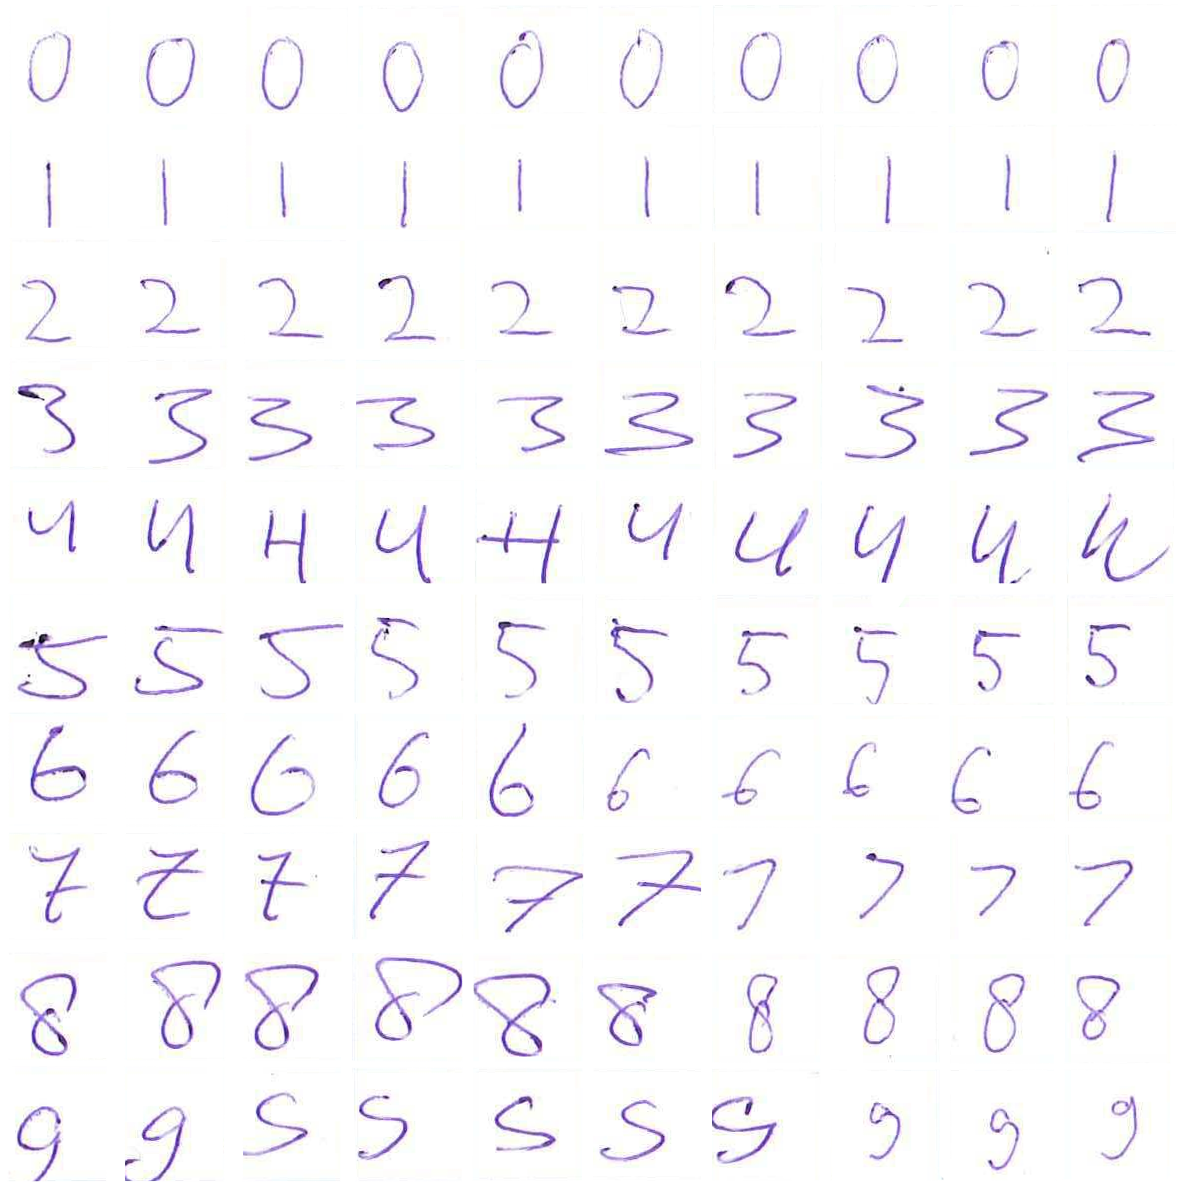
\includegraphics[width=\columnwidth]{images/handwritten.png}
    \caption{Our own handwritten digits}
    \label{fig:handwritten}
\end{figure}

We trained the voted perceptron classifier on 1000 samples for each dataset and
then tested it on our own handwriting.

We did a small amount of preprocessing on our scan. First we extracted the
individual digits from our handwriting. This was pretty easy because the digits
in the figure were well aligned. The image had rgb channels, but we wanted it to
be a boolean image, so in order to get a boolean result, we averaged the rgb
components, to calculate the strength for each pixel and then we tresholded all the
pixels on a value we found by experimentation.

After running the classifier, we found an error rate of 20\%.
Because not all the digits in our handwriting are as clear as the other ones, we
thought it was interesting to make a confusing matrix (in table
\ref{tab:confmatrix}) of our result to detect which digits are the outliers.
We also made a table of error rates (in table \ref{tab:errorrate}).
As can be seen our 7's and 9's are hard for the classifier to recognize, whereas
our 1, 2, 5 and 8 are recognized in all cases.

\begin{table}[H]
    \centering
    \begin{tabular}{|c|cccccccccc | c|}
        \hline 
        True   & \multicolumn{10}{c|}{Estimated Labels} & To-\\
        Label & 0 & 1 & 2 & 3 & 4 & 5 & 6 & 7 & 8 & 9 & tals \\
        \hline
        0 & 9 & 0  & 0  & 0 & 0 & 0  & 0  & 1 & 0  & 0 & 10 \\
        1 & 0 & 10 & 0  & 0 & 0 & 0  & 0  & 0 & 0  & 0 & 10 \\
        2 & 0 & 0  & 10 & 0 & 0 & 0  & 0  & 0 & 0  & 0 & 10 \\
        3 & 0 & 0  & 0  & 8 & 0 & 2  & 0  & 0 & 0  & 0 & 10 \\
        4 & 0 & 0  & 0  & 0 & 9 & 0  & 1  & 0 & 0  & 0 & 10 \\
        5 & 0 & 0  & 0  & 0 & 0 & 10 & 0  & 0 & 0  & 0 & 10 \\
        6 & 0 & 0  & 0  & 0 & 0 & 0  & 10 & 0 & 0  & 0 & 10 \\
        7 & 0 & 2  & 0  & 2 & 0 & 0  & 0  & 6 & 0  & 0 & 10 \\
        8 & 0 & 0  & 0  & 0 & 0 & 0  & 0  & 0 & 10 & 0 & 10 \\
        9 & 3 & 0  & 1  & 2 & 0 & 1  & 0  & 0 & 0  & 3 & 10 \\
        \hline 
        Total & 12 & 12 & 11 & 12 & 9 & 13 & 11 & 7 & 10 & 3 & 100 \\
        \hline 
    \end{tabular}
    \caption{Confusion matrix}
    \label{tab:confmatrix}
\end{table}

\begin{table}
    \begin{tabular}{|c|cccccccccc|}
        \hline
        Class & 0 & 1 & 2 & 3 & 4 & 5 & 6 & 7 & 8 & 9 \\
        \hline
        Error & 1 & 0 & 0 & 3 & 2 & 0 & 1 & 5 & 0 & 8 \\
        \hline
    \end{tabular}
    \caption{Error rate per class}
    \label{tab:errorrate}
\end{table}

\printbibliography

\end{document}

